\documentclass{gshs-hutech}
\usepackage{amsmath,amssymb,amsthm,multirow,dsfont,pifont,graphicx}
\usepackage{graphicx}

\begin{document}
	\begin{center}
		\LARGE A simulation of Hierarchical fragmentation using Processing
	\end{center}

\begin{figure}[h]
	\begin{center}
		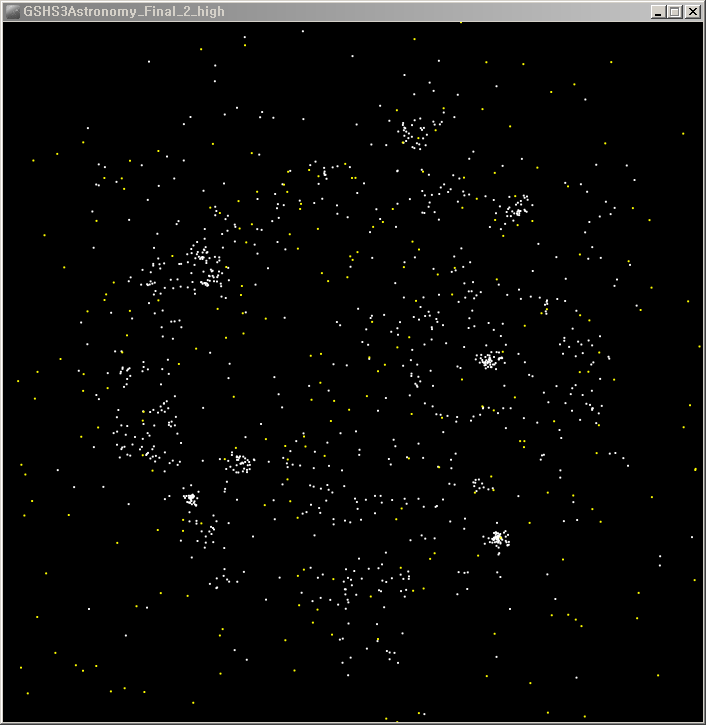
\includegraphics[scale=0.7]{cover.png}
	\end{center}
\end{figure}

\begin{table}[h]
	\begin{center}
		\begin{tabular}{|c|c|c|}
			\hline
			학번&이름&이메일\\
			\hline
			14015&김성윤&clifter0122@naver.com\\
			\hline
			14041&박승원&psw1153@naver.com\\
			\hline
			14061&안형서&danny0122@naver.com\\
			\hline
			14095&임도훈&ehgns0417@naver.com\\
			\hline
			14121&하석민&min990104@naver.com\\
			\hline
		\end{tabular}
		
		Project Participants
	\end{center}
\end{table}
\clearpage
\tableofcontents

\begin{abstract}
우리는 천문학 수업시간에 배운 Hierarchical fragmentation을 직접 프로그래밍을 통해 구현하고자 하였다.

사용한 언어는 Processing이며, 이는 C언어에 비해 물리적 현상의 시각화에 유리하다.

물론 기존에도 Hierarchical fragmentation을 구현한 논문[\ref{bib1}]이 많았지만, 우리는 기존의 것에 비하여 알고리즘의 복잡성을 배제함과 동시에 coolant의 역할을 중요하게 여겨 coolant가 있을때와 없을 때를 서로 비교한 결과, coolant가 있을 때 Hierarchical fragmentation이 더 잘 일어남을 관찰할 수 있었다.

※This document is written with {\LaTeX}, and satisfies 삼성휴먼테크논문대회 requirements
(except the information of authors written above.)

\end{abstract}

\clearpage

\chapter{Simulation}
\section{프로그램 실행 개요 : 박승원 작성}
우리가 만든 프로그램의 실행 순서는, 우선 초기에 맥스웰-볼츠만 분포에 의한 초기 속도를 가진 입자들과 원형으로 균일하게 배치된 입자들이 설정된다. 화면 크기는 700*700pixel 이다. 
입자들은 서로 중력을 통해 상호작용한다. 하지만 두 입자가 20pixel 보다 가까워지면 20pixel 만큼 떨어졌을 때와 같은 중력을 받는다. 이에 대해서는 \ref{gravity}절에서 더 자세히 설명한다.

또한 입자들은 일정 확률로 광자를 방출하며 속도가 느려지는 cooling을 한다. 광자를 방출할 확률은 입자의 속력에 비례하며, 광자는 입자들에 비해 훨씬 빠른 속도로 움직인다. (이러한 수치들을 scaling하는 일 또한 중요하였다. 이에 대해서는 \ref{scaling}절에서 더 자세히 다룬다.) 또한 다른 입자가 방출한 광자를 흡수하여 속도가 빨라지기도 한다.

이 프로그램은 전산학적으로 최적화되지 않아 입자가 n개일때 시간복잡도 $O(n^2)$의 계산을 수행하므로 실행 시간이 매우 느리다. 느린 실행 시간으로는 상황 진행 과정을 살펴보기 힘드므로, 매 frame을 캠쳐하여 프로그램 종료 시 하나의 gif 이미지로 묶었다. 이 gif 파일을 열면 훨씬 빠른 상황 진행 속도로 관찰할 수 있었다.

별개로 cooling 역할을 하는 광자가 매 frame때마다 생기는 개수를 photoncnt.txt로 출력하기도 하였다. 

※원래는 입자끼리 일정 거리 이상 가까워지면 두개가 합쳐지는 void merge()를 제작하여 사용했었으나, 입자의 크기는 원자 수준이므로 이는 부적절하다고 생각되어 주석 처리하였다. \ref{appendix}절의 코드의 주석을 풀고 실행하면 태양계 생성이나 은하생성 과정을 구현할 수 있을 것이다. 


\section{Initial Conditioning : 박승원 작성}
우리가 만들고자 하는 프로그램은, 초기에 위치, 속도가 무작위로 배열된 입자들이 N개 존재하고, 그 입자들이 서로 중력을 주고받음과 동시에 일정한 확률로 광자를 방출하여 속력이 느려지고, 다른 입자가 방출한 광자를 흡수하여 빨라지기도 한다.

우선 내가 수행한 가장 기본적인 역할은, 입자 N개를 700X700 픽셀의 화면에 어떻게 균일하게 배치하며, 초기속도는 어떻게 주어야 하는지 계산하는 코딩을 하는 것이었다. 사실 이것은 우리의 프로그램이 실제 hierachical fragmentation을 구현하는 데에 있어서 상당히 중요한 것이다 - 만약 초기속도를 무작위로 부여하는 데에 실패한다면 입자들이 중앙으로 한번에 몰려들고 나서 다시 퍼지는 단순한 현상이 벌어지거나, 전체 계의 질량중심의 속도가 0이 아니게 되어 입자들의 대부분이 화면 밖으로 나가버리고 말 것이다. 


\subsection{위치 균일}

원래는 입자를 3D로 배치하여 이것들이 움직이는 것을 시각화하고자 하였으나, 아쉽게도 우리가 사용한 프로그래밍 언어 Processing은 그러한 3D plotting에 최적화되어있지 않아 모델링을 2D로 하기로 하였다.

단순히 생각한다면, 입자의 위치를 $(r$cos$\theta,r$sin$\theta)$와 같이 극좌표계로 나타낼때 $r$, $\theta$에 대하여 각각 랜덤 배치하면 된다고 할 것이다. 하지만 그것은 명백한 오류이다. $\theta$에 대해서는 단순히 랜덤 배치하는 것이 맞지만, 
$r$에 대해서도 단순한 랜덤 배치를 한다면, 원점에 가까울수록 단위면적당 입자 수가 많을 것이다. 따라서 단위면적당 입자 수가 균일하려면, 거리 $r$인 곳에 입자가 배치될 확률은 $r$에 비례해야 한다. 거리 $r \sim r+dr$의 영역의 넓이는 $2\pi rdr$로, $r$에 비례하기 때문이다. 

우리에게 주어진 랜덤함수의 기능은, $x$가 출현할 확률이 $P(x)\propto x$와 같이 
$x$에 비례하게 할 수 있지는 않다. 단순히 random(a,b)는 a와 b사이의 실수를 균일한 확률로 준다. 따라서 우리는 동적표(dynamic table)을 만들어 사용해야 한다.

가령 A, B, C가 나올 확률이 각각 1/7, 4/7, 2/7이 되는 동적표를 만든다고 하자. random (0,10000)을 통해 0부터 10000까지의 실수를 얻게 될 때, 표 \ref{dynamic_table}의 맨오른쪽 칸의 ‘범위’와 같이 실수를 대응시키면 된다.

\begin{table}[h]
	\begin{center}
		\begin{tabular}{|c|c|c|c|c|}
			\hline
			문자&원하는 확률&누적&누적*10000&범위\\
			\hline
			A&1/7&1/7&1429&0 - 1429\\
			\hline
			B&4/7&5/7&7142&1429 - 7142\\
			\hline
			C&2/7&1&10000&7142 - 10000\\
			\hline
		\end{tabular}
		
		dynamic\_table
	\end{center}
\end{table} 

이제 본격적으로 입자의 위치를 균일하게 배치시키자. 거리 $r$이 될 확률이 $r$에 비례하면 된다. 따라서, 표 \ref{dynamic_table} 에서의 ‘누적’ 은 따로 배열을 만들어 누적시켜 계산할 필요도 없이, 부정적분에 의하여 ‘누적’은 $r^2$에 비례함을 알 수 있다. 따라서, 
$r$은 $\sqrt{random(0,R^2)}$ 으로 얻으면 된다. (여기에서 $R$은 초기 입자계의 반경이다.)$\theta$는 전에도 언급했듯이 단순히 $random(0,2\pi)$로 얻으면 된다.

※ 3D로 프로그램을 제작할 경우

이 경우 극좌표계는 $(r$sin$\theta $cos$\phi,r$sin$\theta $sin$\phi, r$cos$\theta)$와 같으며, $\phi$에 대해서는 회전대칭이므로 $\phi$는 단순한 랜덤을 사용해도 되지만, $r$의 경우 거리 $r \sim r+dr$의 영역의 부피 $4\pi r^2 dr$, 즉 $r^2$에 비례한 확률로 배치되어야 되며, $\theta$의 경우 반지름 $R$의 구를 생각할 때 $\theta \sim \theta + d\theta$의 영역의 넓이는 $2\pi r$sin$\theta d\theta$이므로 sin$\theta$에 비례하는 확률로 배치되어야 한다.

$r$의 경우 $r^2$을 부정적분하면 $r^3$에 비례하므로 $r=^3 \sqrt{random(0,R^3)}$을 사용하면 되며, $\theta$의 경우 sin$\theta$를 부정적분하면 $-$cos$\theta$이므로, $\theta = $arccos$(random(-1,1))$으로 얻으면 된다.

\subsection{초기속도 부여하기}

속도 역시 속도벡터의 종점을 극좌표계 $(v$cos$\theta,v$sin$\theta)$로 나타내면 된다. 하지만 여기에서 $|\vec{v}|$는 맥스웰-볼츠만 분포를 따라야 한다. $P(v)\propto v^2 e^{-mv^2 / 2kT}$이며, 이것을 부정적분할수는 없다. 따라서 이 경우에는 부득이하게 배열을 만들어 동적표를 직접 만들어야 하며, 랜덤함수를 통해 실수를 얻었을 때 그것이 동적표에서 어느 칸에 해당되는지 찾아야 이를 속도 값에 배치시킬 수 있다.

이 알고리즘의 시간복잡도는 O(동적표의 칸 수 * 입자의 개수)로, 이전에 위치 배열 시의 시간복잡도 O(입자의 개수) 보다 훨씬 커서, 유감스럽게도 프로그램 실행 시작 시 소요되는 대부분의 시간을 차지하게 된다. 

속도의 방향 $\theta$의 경우 위치 배열 때와 마찬가지로 $random(0,2\pi)$를 사용하면 된다.


\section{Gravitational Simulation : 임도훈 작성} \label{gravity}
\subsection{서론}

Hierarchical Fragmentation을 구현할 때 가장 처음 눈에 보이는 것은 수축하는 분자 구름이다. 분자 구름이 수축하기 위해서는 중력이 작용해야 된다. 그러므로 Hierarchical Fragmentation을 구현하는 데에 가장 중요한 알고리즘 중 하나가 중력 알고리즘이라고 할 수 있을 것이다. 그래서 가장 단순하지만 가장 중요한 많은 입자가 뿌려져 있을 때 중력에 의해 입자들이 중심으로 운동하는 즉 분자운이 수축하는 매커니즘을 코딩해서 시각화하는 코드를 제작하였다.
 

\subsection{이론적 배경}

$\vec{F} = G \frac{Mm}{R^3} \vec{R} = m\vec{a}$
($M$은 다른 물체의 질량, $m$은 지금 대상으로 하고 있는 물체의 질량이다.)

이론적으로 위 식이 성립한다. 즉 두 입자의 거리의 제곱에 반비례하고 각 입자의 질량에 비례한다. 그리고 입자간의 거리 방향으로 힘이 작용한다. 수소 분자운을 구현할 경우 매우 많은 입자가 존재하므로 한 입자가 받는 알짜힘을 구하기 위해서는 이 모든 힘의 벡터합을 구해야 한다. 그러기 위해서 중력을 $x$,$y$축방향 힘으로 분해하여 $x$방향 알짜힘과 $y$방향 알짜힘을 구해 $x$,$y$방향 가속도를 구한 다음 그 프레임에서의 속력을 계산해 다음프레임에서는 각 입자의 위치가 어디로 나타나야 하는가를 계산하여 나타내었다. 

\subsection{주요 알고리즘 소개}

\subsubsection{Orbiter Class 의 지정}
Orbiter(float x, float y, float mass)

먼저 각 입자의 정보를 새로운 구조체로 정리하였다. 이 구조체는 입자의 성질을 알아보기 쉽게 정리한 것으로 입자의 $x$좌표, $y$좌표 그리고 그 입자의 질량을 나타내는 구조체이다. 

\subsubsection{void grav의 구성}
\begin{tiny}
void grav(Orbiter [] other)  

    \{
    	
    	float yGrav=0.0;
    	
    	for(int i=0; i \textless other.length; i++)\{
    		
    		if(y \textgreater other[i].y)\{
    			
    			if(dist(other[i].x, other[i].y, x, y)<20) dist=20;
    			
    			else dist=dist(other[i].x, other[i].y, x, y);
    			
    			yGrav-=(mass * other[i].mass) / sq(dist)*abs(other[i].y-y)/dist(other[i].x,other[i].y, x, y) * G;
    			 
    		\}
    		
    		if(y \textless other[i].y)\{
    			
    			if(dist(other[i].x, other[i].y, x, y) \textless 20) dist=20;
    			
    			else dist=dist(other[i].x, other[i].y, x, y);
    			
    			yGrav+=(mass * other[i].mass) / sq(dist)*abs(other[i].y-y)/dist(other[i].x,other[i].y, x, y) * G;
    		\}
    		
    	\}
    	
    	float yAccel=yGrav/mass;
    	
    	yVel += yAccel*0.5;
    	
    	y += yVel*0.5;
    	
    \}
\end{tiny}
    
위의 코드는 중력을 계산하고 중력에 의해서 생기는 가속도와 속도 그리고 다음 프레임에서의 위치를 계산하는 함수이다. 원래 x축 방향과 y축 방향이 모두 있지만 두 코드의 형식은 동일한 관계로 y축 방향을 구한 것만 집어넣었다. 이 코드에서 중요하게 봐야 하는 것은 세 가지이다.

\subsubsection{매우 가까운 두 입자의 거리 처리} \label{two_close_particle}

중력 알고리즘에서의 문제는 매우 가까운 거리에 있는 두 입자에서 나타난다. 두 입자가 매우 가까울 경우 위 식에서 거리 항이 매우 작아져 중력이 기하급수적으로 커지게 된다. 만약에 시간이 연속적이라면 큰 문제는 없을 것이다. 실제 세계에서는 두 입자가 가속되어 서로 반대방향으로 튀어나가는 현상이 없기 때문이다. 하지만 컴퓨터에서의 시간은 불연속적이다. 이때 우리가 이 코드를 실행시킬 경우 이 프레임 간격동안은 직선운동을 시키는 것으로 근사가 되는 것이다. 그렇다면 한 프레임 간격 동안은 직선운동을 한다는 것인데 실제로는 곡선운동을 하고 있으므로 이때 오차가 생기게 되고 이 오차가 점점 쌓이면서 두 입자는 서로 반발력이 작용하는 것처럼 반대방향으로 튕겨나가게 된다. 

\subsubsection{중력 구하기}

이 코드에서 우리는 y방향의 모든 중력벡터의 합을 구한다. 즉, 중력에 작용하는 방향(양의 방향 혹은 음의 뱡향)과 크기를 모두 계산해서 더해야 하는 것이다. 

먼저 방향을 구하기 위해서 처리한 과정은 물체가 있는 곳의 y좌표보다 큰 y좌표에 중력을 가하는 물체가 있으면 양의 방향으로 중력이 가해진다고 처리하였고 그 반대의 경우에는 음의 방향으로 중력이 가해진다고 처리하였다. 

그리고 중력벡터의 크기는 옆 그림에 있는 식을 이용하여 x방향의 힘과 y방향의 힘으로 나누어 그 크기를 계산하였다. 즉 x방향의 중력은 $F_x = G\frac{Mm}{R'^2}\frac{x}{R}$이고 y방향의 중력은 $F_y = G\frac{Mm}{R'^2}\frac{y}{R}$이다.


\begin{figure}[h]
	\begin{center}
		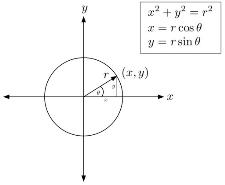
\includegraphics[scale=0.8]{evaluating_gravity.jpg}
		\caption{ }\label{evaluating_gravity}
	\end{center}
\end{figure}

방향성을 나타내는 부분인 cos$(\theta)=\frac{x}{R}$과 sin$(\theta)=\frac{y}{R}$에서는 \ref{two_close_particle}절에서 처리한 $R'$을 사용하지 않고 실제 거리인 $R$로 나타내었는데 그 이유는 방향성을 나타내는 데에 \ref{two_close_particle}절에서 처리한대로 거리를 조작한다면 중력이 작용하는 방향이 변하기 때문이다. 그래서 방향성을 나타내는 데에는 실제 거리를 사용하였다. 

\subsubsection{가속도 및 속력 그리고 위치 구하기}

근사를 하는 알고리즘은 총 3가지를 알아보았다. 첫 번째는 오일러 근사, 두 번째는 verlet 적분법, 그리고 마지막은 Runge-Kutta 근사법이다. 세 근사법은 모두 오차가 존재하지만 그 크기는 오일러 근사, verlet 적분법, 그리고 Runge-Kutta 근사법 순서대로 작아진다. 그렇기 때문에 Runge-Kutta 근사법이나 verlet 적분법을 사용하려 해 보았지만 소요시간 즉 프로그램이 한 프레임을 계산하는데 걸리는 반복 횟수가 증가해서 시간이 오래 걸려 결국 Euler법을 사용하게 되었다. 

그래서 가속도로 속력 그리고 위치를 구하기는 방법을 식으로 표현해 본다면 다음과 같다.

$v(t)=v(t-dt)+a(t)dt$

$x(t)=x(t-dt)+v(t)dt$

가 될 것이다. 이와 같은 방법을 이용하면 이 입자에 작용하는 중력에 의해 속도와 위치가 어떻게 변하는지 계산할 수 있다. 

\subsection{Overall} \label{gravitation_overall}

중력에 의해 분자운이 수축하는 것을 볼 수 있었다. 처음에 예상했던 것은 분자운이 무게중심인 원의 중심으로 수축할 것으로 예상하였지만 불균일하게 일부 부분에 입자들이 중심적으로 입자들이 뭉치는 현상이 존재하였다. 아래에 있는 그림1와 그림 2은 중력에 의해 입자들이 수축하도록 코딩한 코드를 실행시킨 결과이다. 수축하면서 몇몇 부분에 집중적으로 뭉치는 것을 볼 수 있을 것이다. 이를 보고 쿨링 효과나 상수를 맞추는 scaling도 없이 몇몇 부분에 입자들이 뭉치는 효과를 볼 수 있다는 것에서 Hierarchical Fragmentation을 볼 수 있다는 가능성이 있다는 것을 기대하였다. 

하지만 몇몇 부분에 입자들이 뭉치는 효과가 생김에도 불구하고 중력에 의해서 생긴 속도와 뭉친 부분 밖에 있는 입자들의 중력에 의해서 입자들이 다시 흩어지는 것을 볼 수 있었다. 그래서 매우 많은 시간이 흐르면 그림 2처럼 모두 흩어지고 화면 밖으로 나가게 되었다. 그래서 이 알고리즘에 cooling mechanism을 추가하면 에너지의 방출과 수축으로 인해 몇몇 부분에 중심적으로 뭉쳐진 것이 유지될 수 있도록 하면 완벽한 Hierarchical Fragmentation을 볼 수 있을 것이라고 기대하였다. 

그리고 실제 이론대로라면 흩어진 다음에 다시 중심에 모여야 한다. 하지만 내가 만든 코드에서는 한 점에 입자들이 모이는 효과를 발견할 수 없었다. 그래서 이유를 생각해 보다가 상수를 scaling 하여 입자들의 중력의 크기를 조정하면 된다는 것을 알게 되었다.

그래서 cooling mechanism과 상수의 크기를 맞춰주는 scaling을 추가한다면 Hierarchical Fragmentation을 볼 수 있을 것이라고 기대할 수 있었다. 

이를 보정하기 위해서 만일 두 입자가 20pixel 보다 가까운 거리에 있다면 두 입자의 거리를 20pixel로 취급하도록 만들었다. 이렇게 한다면 두 입자가 일정간격 이하로 줄어들었을 때 중력이 기하급수적으로 커져서 입자가 매우 가속하게 되어 서로 반발력이 생기는 것처럼 튕겨나가는 효과는 막을 수 있다. 그래서 이렇게 계산한 거리를 $R'$으로 나타내도록 하자. 

\begin{figure}[h]
	\centering
	\begin{tabular}{cc}
		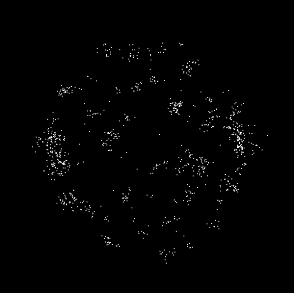
\includegraphics[scale=0.6]{im_fig1.jpg}&
		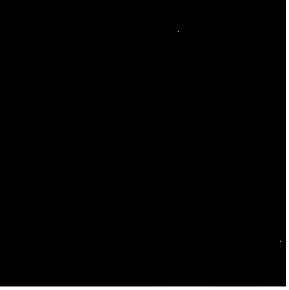
\includegraphics[scale=0.6]{im_fig2.jpg}\\
		그림1 & 그림2
	\end{tabular}
\end{figure}

\section{Role of Coolant during hierarchical fragmentation : 안형서, 하석민 작성} \label{coolant}
\subsection{cooling 도입의 필요성}

본 프로젝트의 목적은 별의 생성과정에서 나타나는 Hierarchical Fragmentation을 직접 구현해 보는 것이다. 초기에 별이 생성될 때 가스나 먼지 입자들이 수축을 한다. 이 때 입자계의 질량은 태양질량의 100000배가 넘을 정도로 많은 물질이 있지만, 실제로 우주에는 질량이 태양질량의 100배 정도 되는 별밖에 존재하지 않는 이유를 제공하는 것이 바로 Hierarchical Fragmentation이다. 

많은 입자들이 뿌려져 있을 때, 이들이 중력에 의해 중심부로 수축을 하는 중력 시뮬레이션은 이미 많이 나와 있다. 그러나 실제로 별이 생길 때는 단순히 중력에 의한 수축 뿐만 아니라, 에너지의 방출, 흡수 등의 기작이 함께 일어나게 된다. 여기서 핵심적인 내용이 cooling이라고 할 수 있다. 따라서 별의 생성 과정을 조금 더 현실과 가깝게 보이기 위해 cooling의 도입이 필요하다.

\subsection{cooling의 이론적인 내용}

\subsubsection{별의 초기 생성 과정(수축)}

Cooling이 별의 생성 과정에서 하는 역할을 알아보기 위해 우선 별의 생성 조건에 대해서 알아보자. 초기에 먼지 등의 입자들이 별로 수축을 하기 위해서는 그 입자계의 중력 포텐셜에너지의 크기가 운동에너지의 총합보다 작아야 한다. 이것이 바로 virial theorem이다. 이를 수식으로 표현하면, $(KE)_{avg}<-\frac{1}{2} (GPE)_{avg}$ 의 조건을 만족할 때, 입자계가 수축할 수 있다. 따라서 초기의 입자들이 위치하는 모양을 구라고 가정했을 때, 입자의 수밀도, 구의 반지름, 질량 등이 결정되면, 그 상태에서 수축을 할 수 있는지의 여부를 알 수 있다. 반대로, 같은 수밀도, 질량을 가진 계가 수축하기 위한 최대 반지름 $R_J$나 같은 수밀도, 반지름을 가진 계가 수축하기 위한 최소 질량
$M_J$를 구할 수도 있다. 이 조건을 따져서, 초기 상태에서 별이 생기기 위한 조건을 구한 것이 바로 Jeans criteria이다. 이를 수식으로 나타내면, $M_J=(\frac{5kT}{\mu m_HG})^{\frac{3}{2}}(\frac{3}{4\pi \rho})^{\frac{1}{2}}$,
$R_J=(\frac{15\pi kT}{4G\rho \mu m_H})^{\frac{1}{2}}$로 표현할 수 있다. 여기서 $T$는 계의 온도, $\mu$는 입자 1개의 평균 분자량, $k$는 볼츠만 상수, $M$은 전체 질량, $\rho$는 밀도, $m_H$는 수소 질량이다.(모든 입자가 수소라고 가정했다.) 여기서는 전체 계가 균일한 밀도를 가지고 온도가 모두 같다고 가정했다. 입자 수가 충분히 많을 때 이와 같이 가정할 수 있다.
 
이제 실제로 일어나는 일에 대해 알아보자. 초기 조건을 만족해서 입자가 수축한다고 가정하자. 중력수축시 계의 밀도와 온도가 증가하게 된다. 그러나 여기서 cooling이 일어나서 온도가 다시 감소하게 된다. 즉, $R_J$의 식에서 분자에 있는 온도의 증가효과보다 분모에 있는 밀도항의 증가효과가 더 크기 때문에 $R_J$는 감소하게 된다. 그리고 실제 계의 반지름 $R$의 감소효과보다 
$R_J$의 감소효과가 더 크기 때문에 계층적으로 수축이 가능하다. 따라서 태양질량의 100000배 정도 되는 큰 별이 존재하지 않는 것이다. 여기서 별이 충분히 식으면 불투명도가 증가하고, 빛이 빠져나가지 못해서 cooling이 더 이상 일어나지 않아 $R$이 $R_J$보다 커져 수축이 중지된다. 여기서 우리는 cooling이 별의 생성과정에서 얼마나 중요한지를 알 수 있다.
 
\subsubsection{cooling의 기작}

이제 cooling이 일어나는 기작에 대해서 알아보자. 우리가 사용한 cooling은 냉매제에 의한 cooling이다. 냉매제에 의한 cooling은 냉매제와 입자의 충돌에 의해 일어난다. 원자와 냉매제가 충돌하게 되면 냉매제가 원자의 에너지를 조금 흡수하고 다시 방출하면서 운동에너지를 빛 에너지로 변환시켜 방출시킨다. 이때, 냉매제의 대표적인 예로는 $C^+$가 있다. 수소 원자가 cooling을 하게 되면, 수소원자가 에너지를 흡수하고 다시 방출해야 한다. 하지만 바닥상태의 수소원자가 에너지를 흡수하려면, 최소 $n=1$에서 $n=2$로 가야하고, 최소 $10.2eV$의 에너지를 흡수해야 한다. 하지만 $C^+$의 경우는 미세구조가 존재하여, $0.01eV$의 에너지도 흡수할 수 있다. 따라서 $C^+$는 운동에너지가 작은 입자의 에너지도 쉽게 흡수하여 빛에너지로 방출할 수 있으므로, $C^+$는 cooling을 효과적으로 할 수 있다.


\begin{figure}[h]
	\begin{center}
		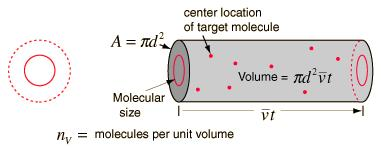
\includegraphics[scale=0.8]{mean_free_path.jpg}
		
		Mean free path에 대한 그림.
	\end{center}
\end{figure}

위의 그림과 같이 면적이 $A$이고 높이가 $vt$인 원통 안에 물질 1이 1개 들어있다고 가정하자. 이 옆에 면적이 $A$이고 높이가 $x$인 원통에 cross section이 $\sigma$인 물질 2가 $N_2$개 있다고 하자. 충돌에 의한 transition이 있을 것이기 때문에 cooling의 빈도를 알기 위해서는 충돌 빈도를 구하는 것이 중요하다. 물질 1 1개가 물질 2와 만날 확률 $p_{12} = \frac{N_2\sigma}{A}=\sigma n_2x$ 이다. (여기서 $n_2=\frac{N_2}{V}={N_2}{Avt}$는 수밀도이다. 여기서는 물질 2의 cross section들이 겹치지 않는다고 가정했다.)

평균 자유 행로(mean free path)는 한 번 충돌할 때까지 움직이는 거리이므로 $p_{12}=1$로 거리는 $l=\frac{1}{n_2\sigma}$이다. 따라서 냉매제와 원자의 평균 충돌 시간은, 즉 평균 자유 시간(mean free time)은 $t=\frac{l}{v}=\frac{1}{n_2\sigma v}=\frac{1}{n\pi r^2v}$이다.여기서 (초당 충돌 횟수)$\propto \frac{1}{t} \propto v$ 임을 알 수 있다.

따라서 원자는 평균적으로 $t$초 마다 한 번씩 cooling에 의해 광자를 방출한다고 생각할 수 있다. 

\subsubsection{Cooling 도입시 우리가 한 가정}

- 냉매제에 의한 cooling을 고려할 때, 냉매제를 입자로 집어넣거나, 냉매제의 밀도를 입자의 밀도에 비례한다는 가정을 통해 할 수도 있었으나, 계산을 줄이고 단순화하기 위해 냉매제의 밀도는 어디든 일정하다고 가정했다.  

- $t$는 mean free time이고 단위시간이 $dt$일때, $dt$동안 원자와 광자가 충돌한 횟수의 확률은 $dt/t$이다. $dt/t$는 사실 기댓값이기 때문에 1을 넘을 수 있는데, 1을 넘을때는 단위시간 동안 항상 한 번 방출하는 것으로 생각한다.

- 원자는 속력에 비례한 일정한 확률로 광자를 먹거나 방출한다.
이는 cooling의 기작에서 평균 충돌 시간이 속력에 비례한다는 결론을 가지고 온 것이다.

-광자들은 일정한 에너지 $E$를 가지고 있다.

-광자를 방출하고 흡수할 때마다 원자는 $E$의 운동에너지를 얻고 잃는다.

-운동량은 고려하지 않으며, 광자를 흡수/방출할 때 운동방향은 그대로로 한다.


\section{Implementation of cooling: 안형서 작성} \label{implementation_cooling} 

먼저, cooling 기작에서 중요한 매개체는 광자이다. 따라서 광자를 구현해야 한다. 광자는 원자와 마찬가지로 속력과 위치를 가지므로 원자와 같이 구현하되, 생성과 소멸이 빈번한 것이 특징이다. 이에 따라서 우리는 쉽게 생성과 소멸이 가능하고, 메모리 낭비가 적은 ArrayList를 이용하였다. 

두 번째로, 확률적으로 광자를 방출하는 것을 구현하였다. 위에서 했던 가정에 따라, 단위시간 마다 각 원자에 대해 확률을 계산한다. 확률은 그 원자의 속력에 비례하게 했으며, 확률 상수를 $p$라고 하고 속력을 $v$라고 하면 $1\sim 1000000$의 정수를 무작위하게 하나 생성한 후, 그 수가 $1000000*p*v$보다 작으면 광자를 방출하도록 만들었다. 원자가 광자를 방출하게 되면, 광자의 에너지 상수 $E$ 만큼의 에너지를 잃도록 하였다. 단, 원자의 운동 에너지가 $E$ 보다 작다면 cooling 기작은 일어나지 않게 하였다. 또, 광자는 무작위의 방향으로 방출되며, 원자의 운동방향은 변하지 않도록 구현하였다.  

다음으로, 원자가 광자를 흡수하는 기작을 구현하였다. 빛의 흡수는 cross section을 상수로 놓고, 광자와 원자 사이의 거리가 특정 거리보다 가까워진다면, 흡수되었다고 판단하여, 광자를 제거하고, 원자의 운동방향은 그대로인 상태로 운동에너지가 E만큼 증가하게 했다. 이 때, 고려해야 할 점이 있었는데, 만약 광자가 생성된 후 바로 광자를 흡수한다고 계산하면, 처음에는 광자와 원자의 위치가 같기 때문에 둘의 거리가 $0$이 되어 광자가 방출되자마자 흡수되어 버린다. 따라서 상수 $photon\_age$ 를 잡아 광자가 방출된지 $photon\_age$ 프레임이 지난 후 부터만 흡수가 가능하도록 만들었다.
 

\section{comparison : 하석민 작성} \label{comparison}

우리가 도입한 cooling의 효과가 어떠한지를 비교해 보자. 그러기 위해서 온도 등 다른 초기 조건은 모두 일정한 상태에서 cooling이 있을 때와 없을 때 수축하는 모양이 어떻게 다른지를 비교해 보아야 한다. 분자구름이 cooling 없이 중력에 의해서만 수축을 하는 것을 관찰하고자 한다면 프로그램 소스코드에서 void cooling()을 주석처리하면 된다.

비록 온도는 scaling을 통해서 200K일 때 가장 Hierarchical Fragmentation이 잘 일어났음을 확인할 수 있었지만, 다른 온도에서도 cooling의 유무가 어떤 역할을 하는지 확인해 보기 위해 크게 다음과 같이 4가지 온도(50K,100K,200K,300K)에서의 수축의 모습을 보았다.

\begin{figure}[h]
	\centering
	\begin{tabular}{cc}
		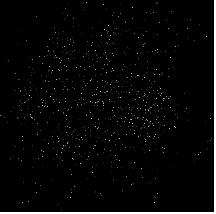
\includegraphics[scale=0.8]{c_1.jpg}&
		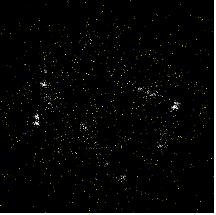
\includegraphics[scale=0.8]{c_2.jpg}\\
		(1) & (2)
	\end{tabular}
\end{figure} 
		
\begin{figure}[h]
	\centering
	\begin{tabular}{cc}
		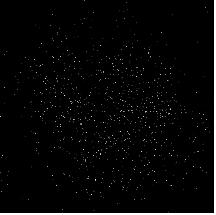
\includegraphics[scale=0.8]{c_3.jpg}&
		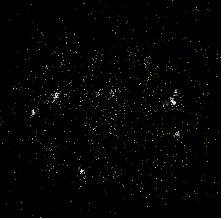
\includegraphics[scale=0.8]{c_4.jpg}\\
		(3) & (4)
	\end{tabular}
\end{figure} 

\begin{table}[h]
	\begin{center}
		\begin{tabular}{|c|c|c|c|}
			\hline
			온도&Not using coolant&Using coolant\\
			\hline
			50K&(1)&(2)\\
			\hline
			100K&(3)&(4)\\
			\hline
		\end{tabular}
	\end{center}
\end{table}

50K, 100K의 낮은 온도에서는 cooling의 효과와 상관없이	분자운이 중력에 의해 중심부로 수축하는 모습을 볼 수 있었다. 그러나 cooling의 효과가 없으면 계층적으로 분열을 하지 않고, 단순히 중심부로 몰리는 경향이 나타났다. 반대로 cooling의 효과를 넣어 보니, 분자운이 중심부로 수축하다가 중간에 계층적으로 분열하는 모습을 볼 수 있었다.


\begin{figure}[h]
	\centering
	\begin{tabular}{cc}
		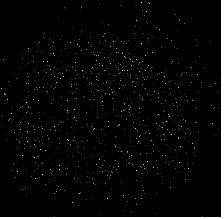
\includegraphics[scale=0.8]{c_5.jpg}&
		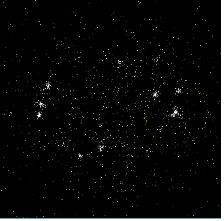
\includegraphics[scale=0.8]{c_6.jpg}\\
		(5) & (6)
	\end{tabular}
\end{figure} 

\begin{figure}[h]
	\centering
	\begin{tabular}{cc}
		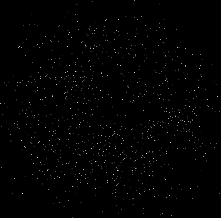
\includegraphics[scale=0.8]{c_7.jpg}&
		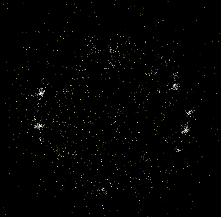
\includegraphics[scale=0.8]{c_8.jpg}\\
		(7) & (8)
	\end{tabular}
\end{figure} 

\begin{table}[h]
	\begin{center}
		\begin{tabular}{|c|c|c|c|}
			\hline
			온도&Not using coolant&Using coolant\\
			\hline
			50K&(5)&(6)\\
			\hline
			100K&(7)&(8)\\
			\hline
		\end{tabular}
	\end{center}
\end{table}

200K, 300K의 온도에서는 cooling 효과가 없을 때, 운동에너지가 중력에 의한 포텐셜 에너지보가 커져서 분자운은 수축하지 않았다. 그러나 cooling의 효과를 추가하니 분자운이 수축을 하고, 또한 Hierarchical Fragmentation도 확인할 수 있었다.

결론적으로, 우리는 가음과 같은 두 가지의 cooling의 효과를 확인할 수 있었다.

1. 분자 구름이 수축할 때 계층적으로 분열할 수 있도록 한다.

2. 처음 주어진 상태로는 수축이 불가능하지만, 이를 수축이 가능하도록 해 준다.

\section{Scaling of Physical Constants : 김성윤 작성} \label{scaling}
\subsection{Scaling의 필요성}

프로그램을 통해 특정 상황을 모델링할 때 상수를 결정하는 것은 무엇보다 중요하다. 이는 특히 천문학과 같은 규모가 큰 상황들을 모델링할 때 더 중요해진다. 천문학에서 기본적으로 입자의 개수는 몰수 단위이며, 거리 역시 서로가 매우 멀리 떨어져 있다. 또한, 천문학적 변화 역시 매우 오랜 시간이 걸리기 마련이다. 간단한 예로, 태양계의 형성에는 약 10억년 이상이 걸리며 상호작용하는 입자들도 매우 많다. 우리가 실제 태양계의 형성을 상수를 그대로 대입하여 보고자 한다면 컴퓨터는 버티지 못할 것이고 (계산량이 너무 많기 때문에), 너무 오랜 시간이 걸리므로 변화를 확인할 수 없을 것이다. 따라서, 상수를 적절히 조절하여 제한된 입자의 개수와 크기, 시간 내에서 우리가 보고자 하는 상황과 가장 유사한 상황을 관측하기 위해 우리는 Scaling을 하여야 한다. 

\subsection{Scaling에서 고려할 점}

이번 프로젝트에서 Scaling은 매우 중요한 문제 중에 하나였다. Scaling을 할 때 나는 3가지 정도의 주요한 요소들을 고려했다. 첫 번째는 시간 간격의 조절이고 두 번째는 cooling rate의 조절, 세 번째는 진스 거리의 조절이었다.

첫 번째는 시간 간격의 조절이다. 실제로 자연상의 모든 변화는 $dt$가 거의 0에 근접하게 변화한다. 따라서, 당연히도 $dt$가 너무 크면 오차가 커지고, 중력 프로그래밍 시에 자주 일어나는 튕김 문제 역시 발생한다. 튕김 문제는 너무 거리가 가까워지는 두 물체 사이에 중력이 과도하게 커져서 둘이 서로 반대방향으로 매우 빠른 속도로 진행하게 되는 문제를 말한다. 튕김 문제를 해결하기 위해서는 거리가 특정 거리 $D$ 이하가 되면 일정한 중력을 받도록 하여서도 해결할 수 있지만, 근본적으로 $dt$를 줄이게 되면 그런 문제는 거의 일어나지 않는다. 하지만, $dt$가 너무 작아지면 Hierarchical Fragmentation을 관찰하는 데 시간이 너무 오래 걸리며, 오히려 입자보다 광자가 더 많아져서 계산량이 급증해 컴퓨터가 버티지 못하게 될 수도 있다. 따라서 적당한 $dt$를 찾는 문제가 중요했다.

두 번째는 cooling rate의 조절이다. cooling rate에는 두 가지 요소가 있는데, 첫 번째 요소는 일반적으로 cooling이 더 잘 일어나게 할 것인지 아닌지를 조절하는 상수이고, 두 번째 요소는 속도가 빠를 때 cooling rate가 증가하는 그 비율을 조절하는 문제이다. 두 번째 요소는 그냥 속도와 cooling rate가 비례하도록 코딩하였으나, 첫 번째 요소를 조절해야 하는 문제가 남아있었다. cooling이 너무 안되면 우리가 보고자 하는 cooling에 의해 확연해지는 Hierarchical Fragmentation을 관찰할 수 없다. 하지만, cooling이 너무 많이 되면 입자들의 속도가 매우 낮아지기 때문에 Hierarchical Fragmentation에 시간이 너무 오래 걸린다. 따라서 적당한 cooling rate를 찾는 문제 역시 중요했다. 비슷한 이유로 cooling이 일어날 때 얼마만큼의 에너지 손실이 있는가 역시도 중요한 문제로 다루었다.

그러나 가장 중요한 것은 진스 거리의 조절이었다. 진스 거리가 너무 크면 cooling의 유무에 관계없이 매우 적은 Hierarchical Fragmentation이 일어난다. cooling이 없어도 Hierarchical Fragmentation이 일어나긴 하지만 그 정도가 매우 적기 때문이다. 또한, 진스 거리가 너무 작으면 아예 입자들끼리 합쳐지지 않는 문제가 있다. 진스 거리를 결정하는 요소에는 세 가지가 있는데, 이들은 밀도, 온도, 중력상수이다. 진스 거리는 온도에 비례하고 밀도와 중력상수에 반비례하는데, 중력상수는 직접 조절할 수 있었다. 그러나 온도와 밀도는 직접 조절할 수 없었기에, 온도를 조절하기 위해 cooling rate를 조절했고, 밀도를 조절하기 위해 cross section을 조절했다. 밀도가 커지면 불투명도가 커지는 효과 때문에 Hierarchical Fragmentation이 더 확연하게 일어나므로 그냥 cross section을 조절하여 불투명도를 인위적으로 조절하였다.  

그 외에 빛의 속도를 조절해야 했다. 빛의 속도를 조절하여 cross section과 함께 불투명도를 조절할 수 있고, 또 빛의 속도가 너무 낮으면 화면상에 입자 수가 너무 많아져 컴퓨터가 버틸 수 없게 되는 문제가 있다.

※ 본 보고서의 scale 순서와 실제 scale 순서는 다릅니다. Scaling을 할 때는 여러 물리량들을 동시에 바꿔가며 최적의 상수들을 찾았지만, 보고서에 그와 같이 쓰게 되면 너무 난잡해질 우려가 있어서 이와 같이 순서를 정해서 설명하였습니다. 

\subsection{$dt$, $m$, $r$, $c$의 Scaling}

사실 이 네가지가 가장 기본적인 물리량이지만, 이와 같은 물리량들까지 굳이 주요하게 scale할 필요는 없었다. 중력을 조절하기 위해서는 G를 조절하면 되며, cooling을 조절하기 위해서는 c와 cross section을 조절하면 되기 때문이다. 따라서 이들은 그냥 기준으로 두었다. m=1로 두었고, r은 좌표상에서의 유클리드 거리로 두었으며, c=100으로 두었다. 다만, dt에 따라서 프로그램의 정확도와 진행시간이 달라지므로 dt를 바꿔가며 가장 적합하다고 판단되는 0.001초로 두었다. dt를 0.001초로 두었을 때 대략 45 $\sim$ 50프레임 사이에서 Hierarchical Fragmentation이 관찰되었으며, cooling을 넣지 않은 상태에 대해서는 그냥 입자들이 하나로 뭉친 모습밖에 관찰할 수 없었다.


\subsection{Jean's length의 Scaling}

사실상 Scaling에서 가장 중요한 부분이 바로 Jean’s length scaling이었다. 이를 scale하므로써 이번 과제에서 cooling이 있을 때와 없을 때에 확연히 드러나는 계층적분열의 차이를 볼 수 있었다. 그 이유는, Jean’s length는 밀도, 중력상수, 온도의 세가지 물리량에 관여하는데, cooling이 있으면 없을 때보다 밀도, 즉 불투명도가 확연히 증가하여 Jean’s length가 cooling이 없을 때보다 더 큰 폭으로 감소하게 되고, 따라서 Hierarchical Fragmentation이 훨씬 더 잘 보이게 된다. 위의 고려할 점 에서는 어떤 물리량들을 어떻게 조절하였는지만 소개하였지만, 여기서는 어떤 상수들을 대입하였을 때 가장 적합하였는지와 그 이유에 대해 설명하겠다.

먼저, Jean’s length가 온도가 높을수록 짧아지는 점, 그리고 온도가 높고 cooling이 없을 땐 실제로는 잘 모이지 않는 점에서 착안하여, 처음에 $T=100K$인 상태에서 온도를 200K정도로까지 올렸다. 200K 근처에서는 Hierarchical Fragmentation의 양상이 비슷했고, 그 이상으로 크게 올리게 되면, cooling을 없앴을 경우에 수축이 거의 일어나지 않고 또 cooling이 있을때도 Jean’s length가 너무 짧아져 Hierarchical Fragmentation이 잘 관측되지 않았기에 200K으로 고정시켰다. 

그 다음으로 cross section을 scale해야 했다. 사실 cross section이 불투명도의 증가, 즉 밀도의 증가를 불러오는 주요한 요인이었기에, cross section을 적당이 크게 하는 것이 중요했다. 만약 cross section이 너무 크다면 역시 cooling의 의미가 사라지게 되기 때문이다. cross section을 100에서 200 정도 사이에 조절해본 결과, 140정도일 때 Hierarchical Fragmentation이 가장 확연하게 드러났다. 

마지막으로 중력 상수는 모이는 시간을 결정하는 데 주요하게 이용했다. 중력 상수가 너무 크면 입자들끼리 너무 빨리 모이게 되기 때문에 Hierarchical Fragmentation을 관찰하기도 전에 한 덩어리가 되어 버리기 때문이다. $G=30$정도로 두었을 때 가장 적합한 결과가 나왔다. 


\subsection{Cooling의 Scaling}

Cooling을 뒤에 구현한 아이디어가 나오겠지만, 랜덤으로 수를 하나 뽑아서 그 수에 cooling rate $r(=t/dt)$과 입자의 속도를 곱한 값이 특정 값 $P$보다 크면 cooling이 일어나도록 하였다. 결국 scale할 것은 $r$과 $P$의 비였는데, $P$를 100000으로 두고 $r$만 조절한 결과, $r=1/500$일때가 가장 적합하였다.

최종적으로 상수들을 정리하자면 다음과 같다.


float dt=0.001;

float t=0.00005;  //  t/dt = probability

float E=50;    // photon's energy

int num=2000;   // orbiter number

float cross\_ section=140;  //  $(collision radius)^2$

float phot\_ age=2;  // the age(frame) that photon starts to collide

float c=100; //  light's speed

float phsize=1;

float planetsize=1;

float G=30;

float R=350;

float T=200;


\chapter{Conclusion} \label{conclusion}

\section{Further Research : 박승원, 하석민 작성} \label{further}

우리의 구현한 시뮬레이션은 coolant이 있을 때에만 Hierarchical Fragmentation이 일어났으므로 Hierarchical Fragmentation에 있어서 coolant의 중요성을 잘 나타낸다고 할 수 있다. 하지만 여러 가지 개선해야 할 한계점들도 있다.

\subsection{Initial Conditioning}
우리는 분자운이 완벽히 균일하게 분포하고, 온도가 일정한다는 가정을 사용하였다. 하지만 실제로는 초기 모든 부분에서 분자운이 입자수밀도가 균일하지 않을 것이고, 모든 곳에서의 온도가 동일하지도 않다. 

또한, 프로그램이 2D로 실행되기 때문에, 3D일 때에 비해 구현되지 않는 사항들이 있을 것이다. 추후에 3D로 구현해 보아야 할 것이다.

\subsection{scaling}
정확한 scaling을 하려면 \ref{scaling}절에서 언급한 scaling의 목적들을 달성하기 위해 현실에서의 physical constants를 서로의 비율을 맞춘 채로 줄이거나 늘려야 하지만, 단순히 프로그램이 잘 실행되기 위해 trial-and-error를 통해서만 상수들을 지정하였었다. 또한, 최종적으로 Hierarchical Fragmentation이 일어나는 데에 소요되는 시간을 실제 값과 비교하여 simulation의 성공도를 보고자 하였으나 실패하였다.

\subsection{Gravitational Method}
우선 우리는 Euler Method를 사용하였고, 두 입자가 가까워질때 튕겨나가는 것을 막기 위해 특정 거리보다 두 입자가 가까워지면 중력이 거리에 무관하게 일정하게 작용하도록 하였다. 하지만 이것은 입자들이 각 부분에서 뭉칠 때 그것이 유지되는 데에 있어서 오류를 야기할 수 있다. 따라서, Euler Method을 사용하며 중력 공식을 변형하기보다는 Verlet Method나 Runge-Kutta 4th Method와 같은 다른 수치미분방정식 풀이법을 사용하여야 한다.

\subsection{Role of Coolant}
우리가 구현한 cooling을 다양하게 실행시켜 보면, 몇 가지 문제점들을 찾을 수 있었다. 
특히 여러 입자들이 좁은 구역에 밀집해서 덩어리와 같이 되었을 때 문제점들을 관측할 수 있다. 여러 입자들이 모였을 때 갑자기 많은 수의 광자가 구면파 형태로 모든 방향으로 지속적으로 방출되는 것을 확인할 수 있었다. 또한, 주위에 다른 영향이 없음에도 불구하고 정지해있었던 입자 뭉치가 갑자기 특정한 방향으로 운동하거나, 갑자기 빨라지는 현상을 관측할 수 있었다. 이것은 에너지 보존 법칙으로 보아도 일어날 수 없는 일이다. 이것은 \ref{gravitation_overall}절에서도 언급하였었다.

\section{Results : 공동작성}
우리는 coolant를 사용할 때와 그렇지 않을 때 Hierarchical fragmentation이 일어나는지를 관찰하였고, 성공적으로 성간운의 Hierarchical fragmentation이 일어날 때 coolant의 중요성을 입증하였다. 우리가 이론적으로만 배웠던 현상을 코딩을 통해 직접 구현해 봄은 큰 의미가 있었고, \ref{further}절에서 보았듯이 많은 한계점들이 있지만, 시간관계상 보완하지 못한 것들은 추후에 더욱 발전시킬 수 있을 것이다. kimhyukssam saranghaeyo!!

\chapter{Bibliography}
\section{Bibloigraphy}
[1] Tsuyoshi Hamada외 5인, {\em42 TFlops Hierarchical N-body Simulations on GPUs with Applications in both Astrophysics and Turbulence}, \label{bib1}

\chapter{Appendix : Processing source code} \label{appendix}
\section{Processing code}
아래의 코드는 최종적으로 완성된 Processing 코드이다. $t$와 $dt$가 서로 뒤바뀌어 있다.
\begin{tiny}

int showsize = 2;

float maxwell[] = new float[100];

float sum=0;

Orbiter [] planet;

ArrayList\textless Photon\textgreater photon =new ArrayList\textless Photon\textgreater();

float dt=0.01;

float t=0.0005;  //  t/dt = probability

float E=30;    // photon's energy

int num=1000;   // orbiter number

float cross\_section=150;  //  (collision radius)\textasciicircum2

float phot\_age=2;  //  the age(frame) that photon starts to collide

float c=100; //  light's speed

float phsize=1;

float planetsize=1;

float G=30;

float R=350;

float T=200;

import gifAnimation.*;

GifMaker gifExport;

PImage gif;

PrintWriter output;

int photoncnt;

void setup()\{

gifExport = new GifMaker(this,"hierachical\_fragmentation.gif");

gifExport.setRepeat(0);

size(700,700);

planet = new Orbiter[num];

for(int i=0; i\textless100; i++)\{

float V;

V=i/T;

maxwell[i]=V*V*exp(-V*V/T);

sum+=maxwell[i];

\}

for(int i=0; i\textless100; i++) maxwell[i]/=sum;

for(int i=1; i\textless100; i++) maxwell[i]+=maxwell[i-1];

for(int i = 0; i \textless planet.length; i++)\{

float r,ran\_theta\_position;

float ran\_v,ran\_theta\_velocity;

r=random(0,122500);

r=sqrt(r);

ran\_v=random(0,1);

int j;

for(j=0; j\textless 100; j++) if(ran\_v\textless maxwell[j]) break;

ran\_v=j/10.0;

ran\_theta\_position=random(0,6.2832);

ran\_theta\_velocity=random(0,6.2832);

planet[i] = new Orbiter(350+r*cos(ran\_theta\_position), 350+r*sin(ran\_theta\_position), planetsize, ran\_v*cos(ran\_theta\_velocity), ran\_v*sin(ran\_theta\_velocity));
\}                                                    //positioning particles\&velocity

noStroke();

smooth();

output = createWriter("photoncnt.txt");

\}//setup simulation screen

void draw()\{

photoncnt = 0;

background(0);

fill(255,255,255);

for(int i = 0; i \textless planet.length; i++)\{

planet[i].grav(planet);                                                                              //gravity of each particle and give them accelation

planet[i].draw();                                                                                             //show particles in screen

//planet[i].keepOnScreen();                                                                                     //to keep particles on screen

\}

fill(255,255,0);

for(int i = 0; i \textless photon.size(); i++)\{

photon.get(i).move();

ellipse((float)photon.get(i).x,(float)photon.get(i).y,showsize*phsize,showsize*phsize);
\}

for(int i = 0; i \textless photon.size(); i++)
\{

	if(photon.get(i).x\textless 0||photon.get(i).x\textgreater width||photon.get(i).y\textless 0||photon.get(i).y\textgreater height)     photon.remove(i);
	
\}

for(int i=0; i\textless num; i++)\{

for(int j=0; j\textless photon.size(); j++)\{

if(photon.get(j).age\textgreater phot\_age)\{

if((planet[i].x-photon.get(j).x)*(planet[i].x-photon.get(j).x)+(planet[i].y-photon.get(j).y)*(planet[i].y-photon.get(j).y)\textless cross\_section)\{

photon.remove(j);

planet[i].kEchange(E);

\}

\}

\}/*

for(int j=0;j\textless i-1;j++)

\{

float temp = sq(planet[i].x-planet[j].x) + sq(planet[i].y-planet[j].y);

if(temp != 0 \&\& sqrt(temp) \textless (sqrt(planet[i].mass) + sqrt(planet[j].mass)) / 4.0) // important!! This determines whether or not the adjacent planets to merge.

\{

planet[i].xVel = (planet[i].mass * planet[i].xVel + planet[j].mass * planet[j].xVel) / (planet[i].mass + planet[j].mass);

planet[i].yVel = (planet[i].mass * planet[i].yVel + planet[j].mass * planet[j].yVel) / (planet[i].mass + planet[j].mass);

planet[i].mass = planet[i].mass + planet[j].mass;

planet[j].mass = 0;

\}

\}*/

\}

gifExport.setDelay(1);

gifExport.addFrame();

output.println(photoncnt);

\}

void keyPressed()

\{

if(key == 32)

\{

gifExport.finish();

output.flush();

output.close();

exit();

\}

\}

class Photon

\{

int age=0;

double x,y,vx,vy;

Photon(double x,double y,double vx,double vy)\{

this.x=x;

this.y=y;

this.vx=vx;

this.vy=vy;

\}

void move()\{

age++;

x+=vx;

y+=vy;

/*

if(x\textless0) \{vx=-vx; x=-x;\}

if(x\textgreater width) \{vx=-vx; x=2*width-x;\}

if(y\textless0) \{vy=-vy; y=-y;\}

if(y\textgreater height) \{vy=-vy; y=2*height-y;\}

*/

\}

\}

class Orbiter                                                                                              //Everything about particle's movement

\{

float x, y, xVel, yVel, mass,dist;

Orbiter(float x, float y, float mass, float xVel, float yVel)

\{

this.x = x;

this.y = y;

this.mass = mass;

this.xVel = xVel;

this.yVel = yVel;


\}                                                                                                    //information of each particle(location\&mass)

/*

void merge(Orbiter [] other)\{

for(int i = 0; i \textless other.length; i++)\{

float temp = sq(other[i].x-x)+sq(other[i].y-y);

if(temp !=0 \&\& sqrt(temp) \textless (sqrt(mass) + sqrt(other[i].mass))/40.0)\{

xVel = (mass * xVel + other[i].mass * other[i].xVel) / (mass + other[i].mass);

yVel = (mass * yVel + other[i].mass * other[i].yVel) / (mass + other[i].mass);

mass += other[i].mass;

planet.remove(i);

\}

\}

\}

*/

void grav(Orbiter [] other)                                                                                          //Gravity of each particles

\{

//

float yGrav=0.0;

for(int i=0; i\textless other.length; i++)\{

if(y\textgreater other[i].y)\{

if(dist(other[i].x, other[i].y, x, y)\textless20) dist=20;

else dist=dist(other[i].x, other[i].y, x, y);

yGrav-=(mass * other[i].mass) / sq(dist)*abs(other[i].y-y)/dist(other[i].x, other[i].y, x, y) * G;

\}

if(y\textless other[i].y)\{

if(dist(other[i].x, other[i].y, x, y)\textless20) dist=20;

else dist=dist(other[i].x, other[i].y, x, y);

yGrav+=(mass * other[i].mass) / sq(dist)*abs(other[i].y-y)/dist(other[i].x, other[i].y, x, y) * G;

\}

\}

float yAccel=yGrav/mass;

yVel += yAccel*0.5;

y += yVel*0.5;


float xGrav=0.0;

for(int i=0; i\textless other.length; i++)\{

if(x\textgreater other[i].x)\{

if(dist(other[i].x, other[i].y, x, y)\textless20) dist=20;

else dist=dist(other[i].x, other[i].y, x, y);

xGrav-=(mass * other[i].mass) / sq(dist)*abs(other[i].x-x)/dist(other[i].x, other[i].y, x, y) * G;

\}

if(x\textless other[i].x)\{

if(dist(other[i].x, other[i].y, x, y)\textless20) dist=20;

else dist=dist(other[i].x, other[i].y, x, y);

xGrav+=(mass * other[i].mass) / sq(dist)*abs(other[i].x-x)/dist(other[i].x, other[i].y, x, y) * G;

\}

\}

float xAccel=xGrav/mass;

xVel += xAccel*0.5;

x += xVel*0.5;


cooling();

\}



void cooling()\{
float v=sqrt(kE());

if(kE()\textgreater E)\{

if(random(0,1000000)\textless1000000*t/dt*v)\{

float theta=random(0,6.283);

Photon pp=new Photon(x,y,c*sin(theta),c*cos(theta));

photon.add(pp);

kEchange(-E);

photoncnt++;

\}

\}

\}



float kE()\{

return (float)(xVel*xVel+yVel*yVel);\}

void kEchange(float e)\{

float r=(kE()+e)/kE();
r=sqrt(r);

xVel*=r;

yVel*=r;

\}

void
keepOnScreen()                                                                                             //to keep all particles on screen

\{

if(x  \textgreater width) xVel=-xVel;

if(y  \textgreater height) yVel=-yVel;

if(x  \textless 0) xVel=-xVel;

if(y  \textless 0) yVel=-yVel;

\}

void draw()\{

ellipse(x, y, showsize*sqrt(mass), showsize*sqrt(mass));

\}

\}



\end{tiny}

\end{document}